\documentclass[12pt]{article}

\usepackage{sbc-template}
\usepackage{graphicx,url}
\usepackage[utf8]{inputenc}
\usepackage{multicol}
\usepackage{listings}
\usepackage{xcolor}
\usepackage{hyperref}
\usepackage{tabto}

\definecolor{codegreen}{rgb}{0,0.6,0}
\definecolor{codegray}{rgb}{0.5,0.5,0.5}
\definecolor{codepurple}{rgb}{0.58,0,0.82}
\definecolor{backcolour}{rgb}{0.95,0.95,0.92}

\lstdefinestyle{mystyle}{
    backgroundcolor=\color{backcolour},   
    commentstyle=\color{codegreen},
    keywordstyle=\color{magenta},
    numberstyle=\tiny\color{codegray},
    stringstyle=\color{codepurple},
    basicstyle=\ttfamily\footnotesize,
    breakatwhitespace=false,         
    breaklines=true,                 
    captionpos=b,                    
    keepspaces=true,                 
    numbers=left,                    
    numbersep=5pt,                  
    showspaces=false,                
    showstringspaces=false,
    showtabs=false,                  
    tabsize=2
}

\lstset{style=mystyle}
   

\sloppy

\title{AED II - Notações de Complexidade}

\author{Luca Ribeiro Schettino Regne}

\begin{document} 

\maketitle

\section{Notação assintótica}
A notação assintótica é um método utilizado para quantificar e definir, através do 
comportamento de algoritmos, o seu nível de complexidade. Para simplificação, essa 
notação desconsidera constantes aditivas e mutiplicativas e leva em consideração 
apenas a \textbf{taxa de crescimento}, isto é, o quão rápido uma função cresce a 
medida que se aumenta o tamanho da entrada.

\subsection{Big-$\Theta$}
Na definição de $\Theta(n)$ são utilizados limites lineares para o tempo de execução, 
sendo que, quando n fica grande o bastante, o tempo de execução é de pelo menos $k_1 \cdot n$
e, no máximo, de $k_{2} \cdot n$ para quaisquer constantes $k_{1}$ e $k_{2}$. Sendo assim 
temos o seguinte cenário $\Theta(n)$:

\begin{center}
    $ k_{2} \cdot n > \Theta(n) > k_{1} \cdot n$\\
    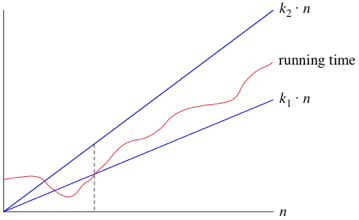
\includegraphics[width=0.5\textwidth]{images/theta_n.png}
\end{center}

\subsection{Big-O}
Diferente da $\Theta(n)$ na notação chamado Big O, ou Grande-O, é utilizado quando se 
deseja encontrar limites assintóticos superiores, ou seja, é traçado apenas o pior caso.

\begin{center}
    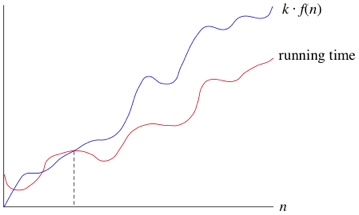
\includegraphics[width=0.5\textwidth]{images/bigO_n.png}\\    
\end{center}

\subsection{Big-$\Omega$}
De maneira contrária ao Big-O a notação Big-$\Omega$ defini apenas um limite inferior.
Então podemos concluir que, seja um tempo de execução $\Omega(f(n))$, para um n suficientemente 
grande, ele será ao menos $k \cdot f(n)$ para uma constante qualquer.\\

\begin{center}
    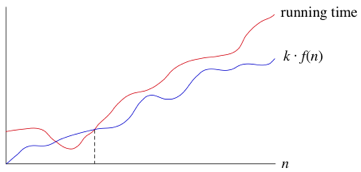
\includegraphics[width=0.5\textwidth]{images/omega_n.png}\\   
\end{center}

\section{Exercícios Resolvidos}

\subsection{Exercício Resolvido 1}
\begin{lstlisting}[language=C]
  ...
  a--;
  a -= 3;
  a = 1 - 2;
\end{lstlisting}
$O(1)$\\
$\Theta(1)$\\
$\Omega(1)$\\


\subsection{Exercício Resolvido 2}
\begin{lstlisting}[language=C]
  ...
  if(a + 5 < b + 3)
    i++;
    ++b;
    a += 3;
  } else {
    j++;
  }
\end{lstlisting}
$O(1)$\\
$\Theta(1)$\\
$\Omega(1)$\\

\subsection{Exercício Resolvido 3}
\begin{lstlisting}[language=C]
  ...
  if(a + 5 < b + 3 || c + 1 < d + 3)
    i++;
    ++b;
    a += 3;
  } else {
    j++;
  }
\end{lstlisting}
$O(1)$\\
$\Theta(1)$\\
$\Omega(1)$\\

\subsection{Exercício Resolvido 4}
\begin{lstlisting}[language=C]
  ...
  for(int i = 0; i < 4; i++){
    a--;
  }
\end{lstlisting}
$O(1)$\\
$\Theta(1)$\\
$\Omega(1)$\\

\subsection{Exercício Resolvido 5}
\begin{lstlisting}[language=C]
  ...
  for(int i = 0; i < n; i++){
    a--;
    b--;
  }
\end{lstlisting}
$O(n)$\\
$\Theta(n^2)$\\
$\Omega(1)$\\

\subsection{Exercício Resolvido 6}
\begin{lstlisting}[language=C]
  ...
  int i =0, b = 10;
  while(i < 3){
    i++;
    b--;
  }
\end{lstlisting}
$O(1)$\\
$\Theta(1)$\\
$\Omega(1)$\\

\subsection{Exercício Resolvido 7}
\begin{lstlisting}[language=C]
  ...
  for(int i = 3; i < n; i++){
    a--;
  }
\end{lstlisting}
$O(n)$\\
$\Theta(n)$\\
$\Omega(n)$\\

\subsection{Exercício Resolvido 8}
\begin{lstlisting}[language=C]
  int a = 10;
  ...
  for(int i = 0; i < 3; i++){
    for(int j = 0; j < 2;j++){
      a--;
    }
  }
\end{lstlisting}
$O(1)$\\
$\Theta(1)$\\
$\Omega(1)$\\

\subsection{Exercício Resolvido 9}
Calcule o número de multiplicações que o código abaixo realiza:
\begin{lstlisting}[language=C]
  ...
  for(int i = n; i < 0; i /= 2){
    a *= 2;
  }
\end{lstlisting}
$O(\log_{2}n)$\\
$\Theta(\log_{2}n)$\\
$\Omega(1)$\\

\subsection{Exercício Resolvido 10}
\begin{lstlisting}[language=C]
  i = 0;
  
  while (i < n){
    i++;a--;
    b--;
    c--;
  }
  
  for (i = 0;  i < n; i++){
    for (j = 0;  j < n; j++){
      a--;
      b--;
    }
  }
\end{lstlisting}
$O(n^3)$\\
$\Theta(n^3)$\\
$\Omega(n)$\\

\subsection{Exercício Resolvido 11}
Encontre o menor valor em um array de inteiros
\begin{lstlisting}[language=C]
  int min = array[0];
  
  for (int i = 1; i < n; i++){
    if (min > array[i]){
      min = array[i];
    }
  }
\end{lstlisting}
$O(n)$\\
$\Theta(n)$\\
$\Omega(1)$\\

\section{Exercícios}

\begin{multicols}{4}
  [
    \subsection{Exercício 1}
  ]
  a) $2^{0} = 1$ \\
  b) $2^{1} = 2$ \\
  c) $2^{2} = 4$ \\
  d) $2^{3} = 8$ \\
  e) $2^{4} = 16$ \\
  f) $2^{5} = 32$ \\
  g) $2^{6} = 64$ \\
  h) $2^{7} = 128$ \\
  i) $2^{8} = 256$ \\
  j) $2^{9} = 512$ \\
  k) $2^{10} = 1024$ \\
  l) $2^{11} = 2048$ \\
  \end{multicols}
  $O(1)$ - $\Theta(1)$ - $\Omega(1)$

\begin{multicols}{4}
  [
    \subsection{Exercício 2}
  ]
  a) $\log{2048} = 11$ \\
  b) $\log{1024} = 10$ \\
  c) $\log{512} = 9$ \\
  d) $\log{256} = 8$ \\
  e) $\log{128} = 7$ \\
  f) $\log{64} = 6$ \\
  j) $\log{32} = 5$ \\
  h) $\log{16} = 4$ \\
  i) $\log{8} = 3$ \\
  j) $\log{4} = 2$ \\
  k) $\log{2} = 1$ \\
  l) $\log{1} = 0$
\end{multicols}
$O(1)$ - $\Theta(1)$ - $\Omega(1)$


\begin{multicols}{4}
  [
    \subsection{Exercício 3}
  ]
  a) $\lceil 4,01 \rceil = 5$ \\
  b) $\lfloor 4,01 \rfloor = 4$ \\
  c) $\lceil 4,99 \rceil = 5$ \\
  d) $\lfloor 4,99 \rfloor = 4$ \\
  e) $\lceil \log{16} \rceil = 4$ \\
  f) $\lfloor \log{16} \rfloor = 4$ \\
  g) $\log{17} = 4.08$ \\
  h) $\lceil \log{17} \rceil = 4$ \\
  i) $\lfloor \log{17} \rfloor = 5$ \\
  j) $\log{15} = 3.90$ \\
  k) $\lceil \log{15} \rceil = 3$ \\
  l) $\lfloor \log{15} \rfloor = 4$ \\
\end{multicols}
$O(1)$ - $\Theta(1)$ - $\Omega(1)$\\

  
\subsection{Exercício 4}
  a) $f(n) = n \\
  O(n) - \Theta(n) - \Omega(1)$\\ \\
  b) $f(n) = n^{2} \\
  O(n^{2}) - \Theta(n^{2}) - \Omega(n)$\\ \\
  c) $f(n) = n^{3} \\
  O(n^{3}) - \Theta(n^{3}) - \Omega(n^{2})$\\ \\
  d) $f(n) = sqrt(n) \\
  O(n^{1/2}) - \Theta(n^{1/2}) - \Omega(n^{1/4})$\\ \\
  e) $f(n) = \lg{n} = \log_{2}{n} \\
  O(\log_{2}{n}) - \Theta(\log_{2}{n}) - \Omega(1)$\\ \\
  f) $f(n) = 3n^{2} + 5n - 3 \\
  O(n^{2}) - \Theta(n^{2}) - \Omega(n)$\\ \\
  g) $f(n) = -3n^{2} + 5n - 3 \\
  O(n^{2}) - \Theta(n^{2}) - \Omega(n)$\\ \\
  h) $f(n) = |-n^{2}| \\
  O(n^{2}) - \Theta(n^{2}) - \Omega(n)$\\ \\
  i) $f(n) = 5n^{4} + 2n^{2} \\
  O(n^{4}) - \Theta(n^{4}) - \Omega(n^{3})$\\ \\
  j) $f(n) = n * \lg{(n)} \\
  O(n \cdot lg(n)) - \Theta(n \cdot lg(n)) - \Omega(lg(n))$\\


\subsection{Exercício 5}
\begin{lstlisting}[language=C]
  ...
  int i = 10;
  while(i >= 7){
    i--;
  }
\end{lstlisting}
$O(1)$\\
$\Theta(1)$\\
$\Omega(1)$\\

\subsection{Exercício 6}
\begin{lstlisting}[language=C]
  ...
  for(int i = 5; i >- 2; i--){
    a--;
  }
\end{lstlisting}
$O(1)$\\
$\Theta(1)$\\
$\Omega(1)$\\

\subsection{Exercício 7}
\begin{lstlisting}[language=C]
  ...
  for (int i = 0; i < 5; i++){
    if (i % 2 == 0){
      a--;
      b--;
    } else{
      c--;
    }
  }
\end{lstlisting}
$O(1)$\\
$\Theta(1)$\\
$\Omega(1)$\\


\subsection{Exercício 8}
\begin{lstlisting}[language=C]
  ...
  for (int i = 0; i < n; i++){
    for (int j = 0; j < n; j++){
      a--;
    }
  }
\end{lstlisting}
$O(n^2)$\\
$\Theta(n^2)$\\
$\Omega(n)$\\

\subsection{Exercício 9}
\begin{lstlisting}[language=C]
  ...
  int i = 1, b = 10;
  while (i > 0){
    b--;
    i = i >> 1;
  }
  i = 0;
  while (i < 15){
    b--;
    i += 2;
  }
\end{lstlisting}
$O(1)$\\
$\Theta(1)$\\
$\Omega(1)$\\

\subsection{Exercício 10}
Calcule o número de multiplicações que o código abaixo realiza:
\begin{lstlisting}[language=C]
  ...
  for (int i = 0; i < n; i++)
    for (int j = 0; j < n - 3; j++)
      a *= 2;
\end{lstlisting}
$O(n^2)$\\
$\Theta(n^2)$\\
$\Omega(n^2)$\\

\subsection{Exercício 11}
Calcule o número de multiplicações que o código abaixo realiza:
\begin{lstlisting}[language=C]
  ...
  for (int i = n - 7; i >= 1; i--)
    for (int j = 0; j < n; j++)
      a *= 2;

\end{lstlisting}
$((n - 7) - 1) * (n) = n * (n - 8)$\\
Serão realizadas n*(n-8) multiplicações.

\subsection{Exercício 12}
Calcule o número de multiplicações que o código abaixo realiza:
\begin{lstlisting}[language=C]
  ...
  for (int i = n; i > 0; i /= 2)
      a *= 2;

\end{lstlisting}
Serão realizadas $\log_{2}{n} + 1$ multiplicações.

\subsection{Exercício 13}
Calcule o número de multiplicações que o código abaixo realiza:
\begin{lstlisting}[language=C]
  ...
  for (int i = n+4; i > 0; i >>= 1)
    a *= 2;
\end{lstlisting}
Serão realizadas $\log_{2}{n+4}$ multiplicações.

\subsection{Exercício 14}
Calcule o número de multiplicações que o código abaixo realiza:
\begin{lstlisting}[language=C]
  ...
  for (int i = n - 7; i >= 1; i--)
    for (int j = n - 7; j >= 1; j--)
      a *= 2;

\end{lstlisting}
Serão realizadas $(n - 7)^2$ multiplicações.

\bibliographystyle{sbc}
\bibliography{sbc-template}

\subsection{Exercício 15}
Calcule o número de multiplicações que o código abaixo realiza:
\begin{lstlisting}[language=C]
  ...
  for (int i = n + 1; i > 0; i /= 2)
    a *= 2;
\end{lstlisting}
Serão realizadas $(\lg{n+1}2$ multiplicações.

\bibliographystyle{sbc}
\bibliography{sbc-template}

\subsection{Exercício 16}
Calcule o número de multiplicações que o código abaixo realiza:
\begin{lstlisting}[language=C]
  ...
  for (int i = n; i > 1; i /= 2)
    a *= 2
\end{lstlisting}
Serão realizadas $\lg{n}$ multiplicações.

\bibliographystyle{sbc}
\bibliography{sbc-template}

\subsection{Exercício 17}
Calcule o número de multiplicações que o código abaixo realiza:
\begin{lstlisting}[language=C]
  ...
  for (int i = 1; i < n; i *= 2)
    a *= 2;
\end{lstlisting}
Serão realizadas $(\sqrt{n}*2)$ multiplicações.

\subsection{Exercício 18}
Calcule o número de multiplicações que o código abaixo realiza:
\begin{lstlisting}[language=C]
  ...
  for (int i = 1; i <= n; i*= 2)
    a *= 2;
\end{lstlisting}
Serão realizadas $((\sqrt{n}+1)*2)$ multiplicações.

\bibliographystyle{sbc}
\bibliography{sbc-template}

\end{document}
